\subsection{Pruebas Individuales de Componentes con Arduino }
\par \noindent
Todas las pruebas serán utilizando un arduino nano; ya que permite una integración sencilla con un breadboard y sera el que utilizaremos en nuestro prototipo final. Empezaremos con el sensor de temperatura DS18B20.

\subsubsection{Arduino y DS18B20}
\par 
Si leemos detenidamente el datasheet del DS18B20 podemos encontrar que es mas complejo que un simple termopar para medir la temperatura. Cuenta en su forma de sonda con distintos circuitos integrados que permiten la facil integración con arduino. El DS18B20 utiliza tres alambres. Uno para la alimentación de 5V, otro para tierra y uno de información o data. Este ultimo es conectado a traves de una resistencia de 4.7K ohmnios en parallelo con una alimentación de 5V y cualquier pin digital de arduino. 

\begin{figure}[H]
	\centering
	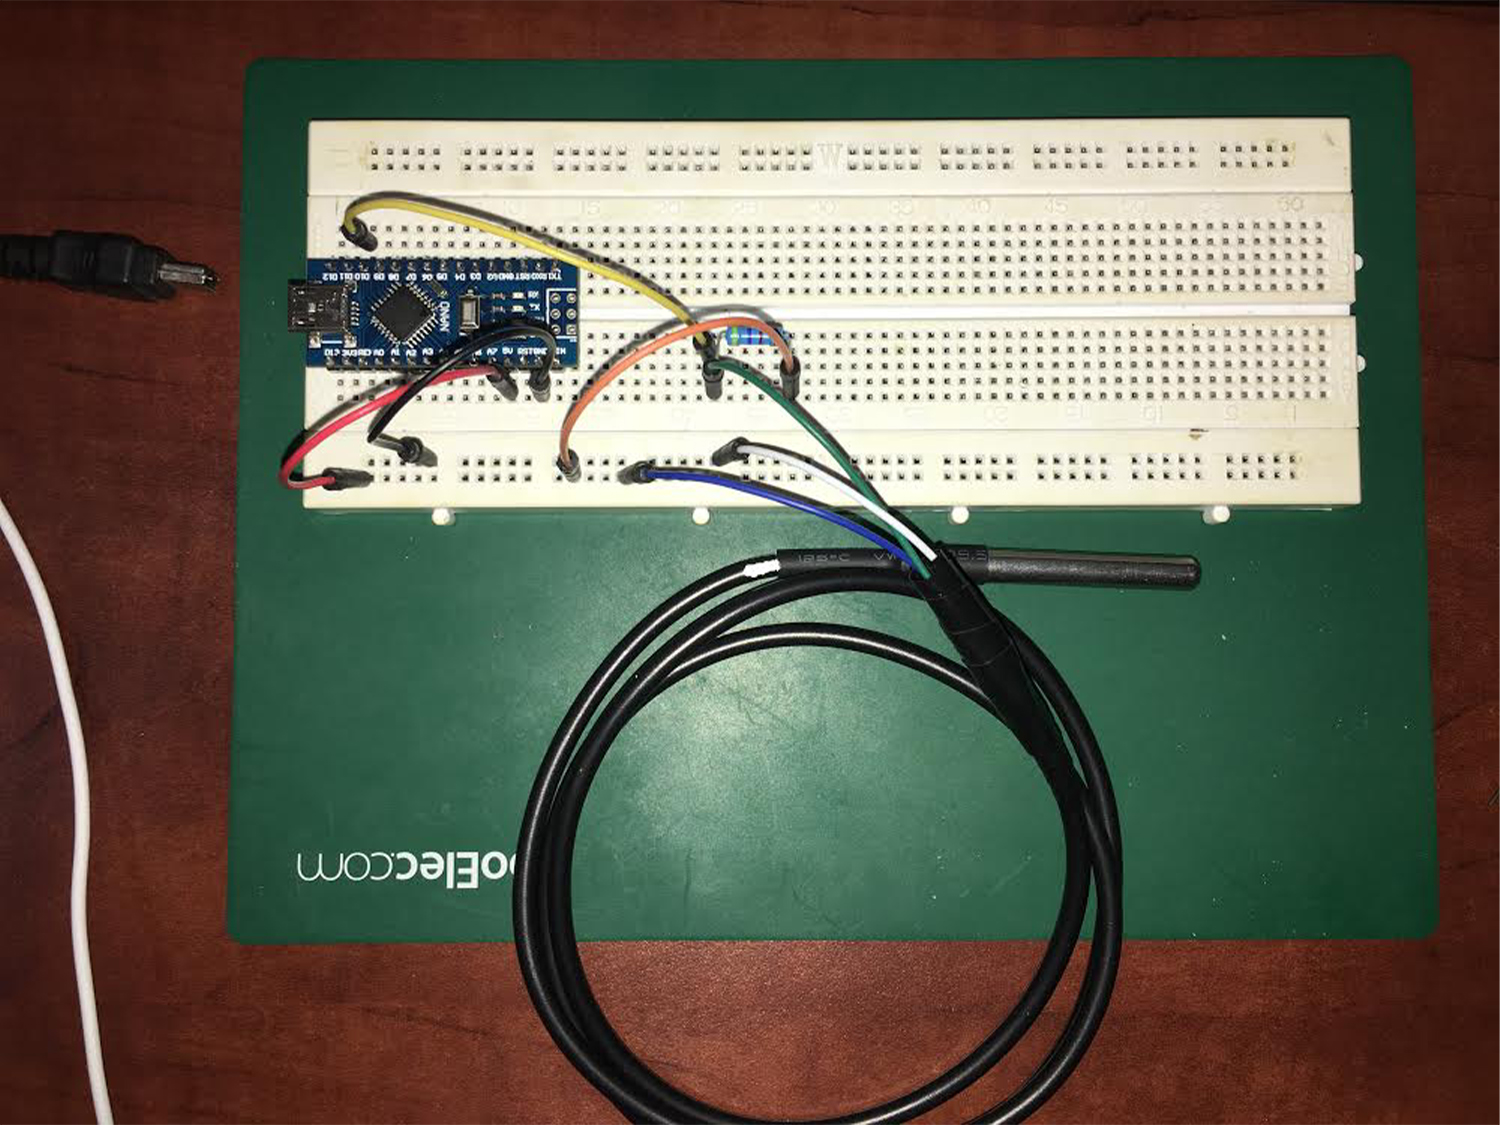
\includegraphics[width=0.65\linewidth]{pruebas1.jpg}
	\caption{Conexión Sencilla entre Arduino Nano y Sensor de Temperatura DS18B20}
\end{figure}

\par \noindent
En la imagen anterior hemos seleccionado el pin digital 10 para enviar la información y vemos como el sensor es conectado a la salida de 5V del Arduino y su respectivo GND, adicional vemos una resistencia de 4.7K entre el cable de DATA del sensor y una conexión al pin 10. 

\par \noindent
Ahora utilizando el software platformio, el entorno de desarrollo que utilizaremos para programar la placa arduino, escribiremos un codigo de prueba. Para ellos necesitaremos de dos librerias: OneWire \cite{onewire-github} y DallasTemperature \cite{dallas-github}. El código de prueba seria el siguiente: \\

\begin{lstlisting}[language=C++, caption={Codigo Ejemplo para DS18B20}, captionpos=b]
#include <Arduino.h>
#include <OneWire.h>
#include <DallasTemperature.h>

#define ONE_WIRE_BUS 10

OneWire oneWire(ONE_WIRE_BUS);
DallasTemperature sensors(&oneWire);

void setup(){
Serial.begin(9600);
sensors.begin();
}


void loop(){
Serial.print("Requesting temperatures...");
sensors.requestTemperatures(); 
Serial.println("DONE");
Serial.print("Temperature:");
Serial.println(sensors.getTempCByIndex(0));
delay(1000);
}
\end{lstlisting}

\par \noindent
El codigo anterior puede ser encontrado como uno de los ejemplos que trae la librería DallasTemperature[30] bajo el nombre "Simple.pde" y puede inspeccionado por cualquier editor de texto. El código basicamente es crear una instancia de la clase OneWire y esa instancia colocarla como argumento dentro del objeto "sensors". En la función setup (se ejecuta una sola vez). Se inicializa el puerto serial a 9600 baudios y se inicializa el objeto "sensors" de clase DallasTemperatures. En la funcion loop, se ejecuta toda la función, desde el inicio hasta el  final, una y otra vez; hasta que se apague el micro-controlador. Se imprime en la terminal de la computadora y se ejecuta la funcion "requestTemperatures" que llama todos los posibles DS18B20 que se encuentren en el mismo bus. Por ultimo se imprime en la terminal de la computadora el resultado de la funcion "getTempCByIndex" donde si esta conectado un DS18B20 retorna la temperatura captura en grados celsius; en caso tal de no encontrarse ningun DS18B20 en el circuito, el valor retornado es "-127" constante de nida en la libreria DallasTemperature.

\par \noindent
Una vez hayamos subido el codigo a nuestro Arduino, debemos validar que el sensor funcione correctamente, pero ¿cómo? Conectado el Arduino a nuestra computadora utilizaremos el puerto serial de nuestro entorno de desarrollo. Si estamos utilizando el IDE de arduino, basta con hacer clic en la barra superior la opcion "herramientas" y seleccionar "Monitor Serial". Como nosotros estamos utilizando Platformio como IDE, basta con seleccionar en la barra de herramientas "Platformio", la opción "Serial Monitor". Esencialmente lo que hace esa opción es escribir en nuestra terminal el comando "pio device monitor  port COM5" y con eso podemos comunicarnos con nuestro Arduino a través de un puerto Serial. En la  gura 4.2, podemos visualizar el resultado del código 4.1, en ejecución por el microcontrolador.

\begin{figure}[H]
	\centering
	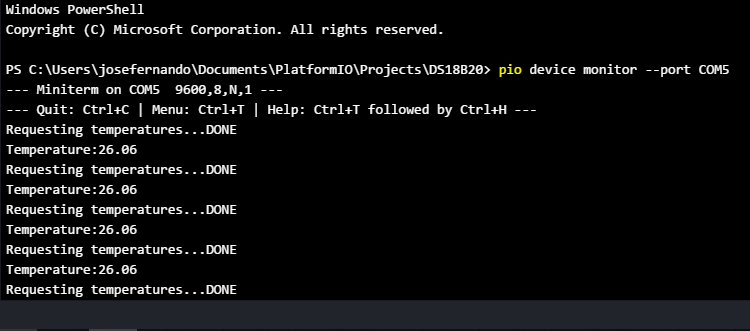
\includegraphics[width=\linewidth]{pruebas2.png}
	\caption{Terminal de windows visualizando temperatura capturada por sensor DS18B20, a través de comunicación serial.}
\end{figure}

\par \noindent
Hemos comprobado lo sencillo que es capturar mediciones de temperatura en tiempo real. Sin embargo no es práctico para el usuario final tener que cargar una computadora, conectar el Arduino y abrir una terminal. Aquí es donde necesitamos la pantalla LCD ILI9348.

\subsubsection{Arduino y Pantalla LCD ILI9341}
\par 
La realidad es que los datasheets de las pantallas LCD son complejas, esto es debido a que se explica más como el controlador de la pantalla interactúa con el LCD. Lo único que pudimos determinar es que la pantalla tolera una alimentación de 5V; pero, el controlador solamente utiliza una lógica de 3.3V. Teniendo en cuenta esto procedimos a conectar la pantalla utilizando divisores de voltaje (resistencias en serie); no obstante, el resultado no fue positivo.

\par \noindent
Por suerte el blog de educ8s.tv\cite{edu8tv} tiene una guía para utilizar la pantalla ILI9341,curiosamente utiliza resistores de 10K en series para las conexiones, a pesar de que las resistencia en serie no disminuyen el voltaje de los pines de Arduino. Conectamos la pantalla LCD ILI9341 a nuestro Arduino según la guía, quedando como se ve en la  gura 4.3

\par \noindent
El controlador de esta pantalla utiliza el bus SPI del Arduino, SPI por sus siglas en inglés es Serial Pheripheral Interface, el cual es un interfaz de bus comunmente utilizado para enviar información entre microcontroladores, sensores, tarjetas SD y otros microcontroladores. Esto quiere decir que las conexiónes de nuestra pantalla estan definidas hacia los pines digitales 13, 12 y 11 para poder comunicarse correctamente con el Arduino.

\begin{figure}[H]
	\centering
	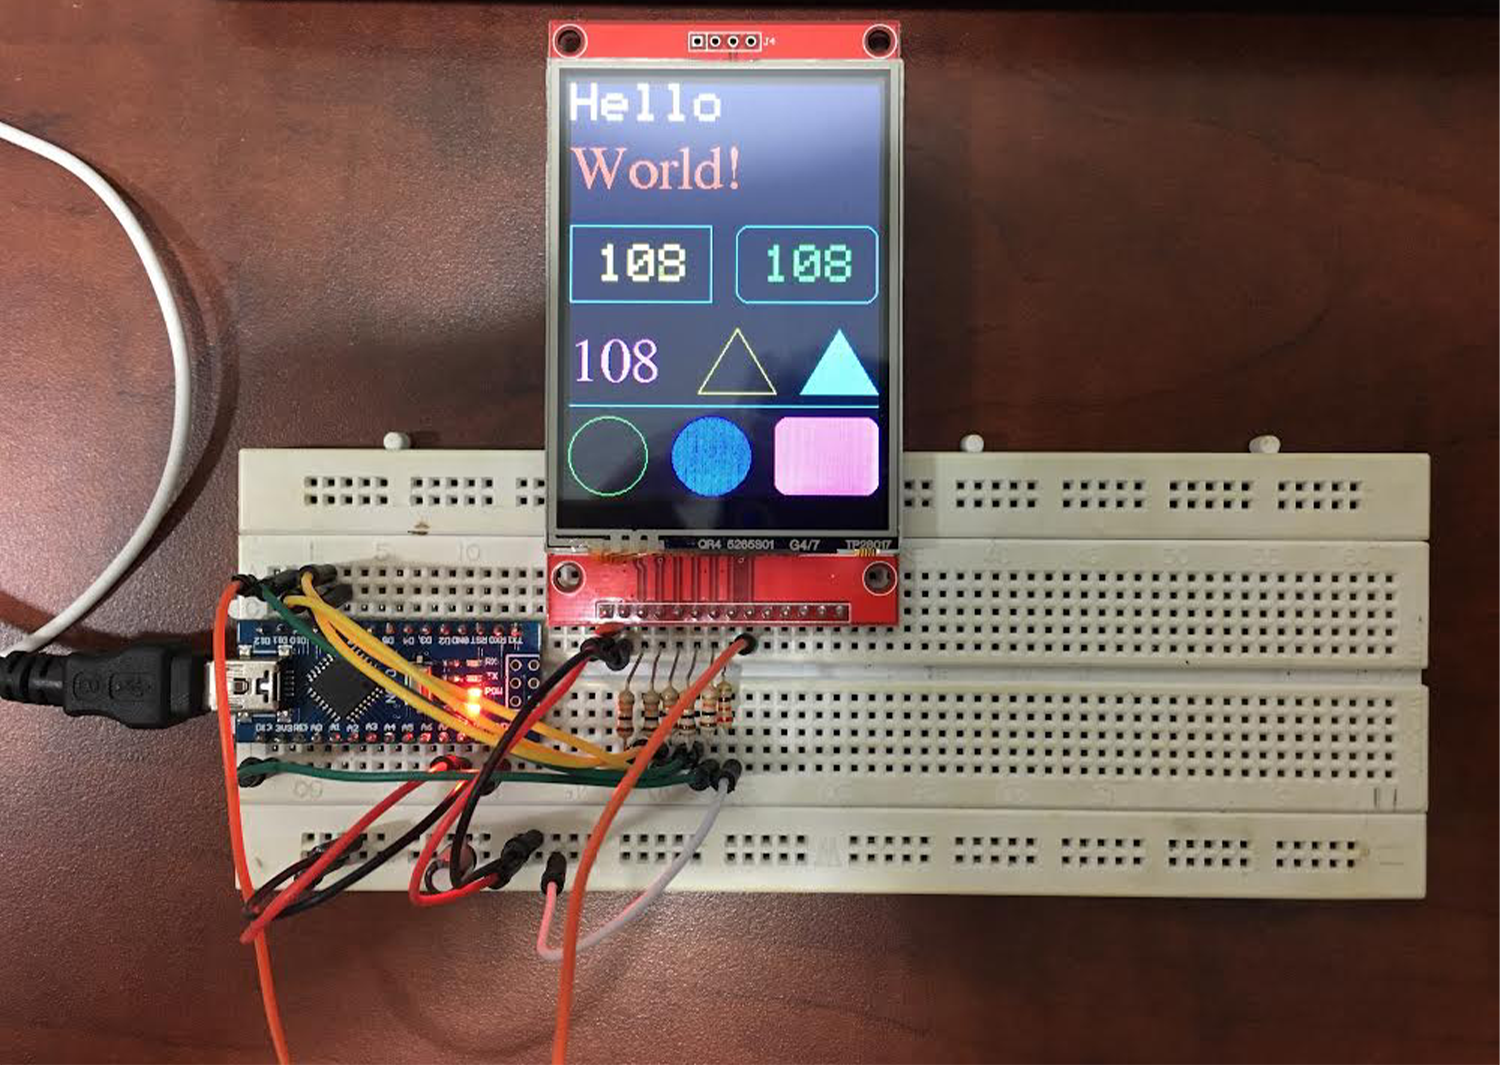
\includegraphics[width=0.8\linewidth]{pruebas3.png}
	\caption{Conexión entre Arduino y LCD ILI9341, utilizando resistencias de 10K en serie.}
\end{figure}

\clearpage

\par \noindent
Cabe a destacar que el circuito de la figura 4.3, utiliza dos componentes pasivos adicionales a las resistencias. Estos son dos capacitores, uno electrolítico de 10 uF, ayuda a filtrar frecuencias bajas y otro de cerámica de 1nF el cual ayuda a filtrar altas frecuencias. El conjunto de ambos brinda una fuente de poder estable a la pantalla LCD.

\par \noindent
La pantalla cuando es conectada al Arduino solamente despliega la luz de fondo blanca de la pantalla. Para programar los pixeles a utilizar en la pantalla debemos utilizar dos librerías: Adafruit\_ILI9341\cite{adafruit-lcd} y Adafruit-GFX-Library\cite{adafruit-gfx} ambos de los mismos desarrolladores de Adafruit, es una compañía de hardware de código abierto y es uno de los principales contribuidores del proyecto Arduino. Utilizamos uno de los códigos ejemplos que vienen con las librerías para verificar el funcionamiento de la pantalla como en la figura 4.3

\begin{lstlisting}[language=C++, caption={Codigo Ejemplo para pantalla LCD ILI9341}, captionpos=b]
#include <Arduino.h>
#include "SPI.h"
#include "Adafruit_GFX.h"
#include "Adafruit_ILI9341.h"

#define TFT_DC 9
#define TFT_CS 10
#define TFT_RST 8
#define TFT_MISO 12
#define TFT_MOSI 11
#define TFT_CLK 13

Adafruit_ILI9341 tft = Adafruit_ILI9341(
TFT_CS, 
TFT_DC, 
TFT_MOSI, 
TFT_CLK, 
TFT_RST, 
TFT_MISO);

#include <Fonts/FreeSerif24pt7b.h>

int Variable1;  

void setup(){

tft.begin();
tft.fillScreen(0x0000);
tft.setTextWrap(false);

tft.setCursor(0, 0);
tft.setTextColor(0xFFFF);
tft.setTextSize(4);
tft.println("Hello");

tft.setFont(&FreeSerif24pt7b);
tft.setTextSize(0);

tft.setCursor(0, 80);
tft.setTextColor(0xF800);
tft.println("World!");

tft.setFont();

tft.drawRect(0, 110, 110, 60, 0x07FF);
tft.drawRoundRect(129, 110, 110, 60, 10, 0x07FF);
tft.drawTriangle(100,240,    130,190,    160,240, 0xFFE0);
tft.fillTriangle(179,240,    209,190,    239,240, 0x07FF);
tft.drawLine(0, 250, 239, 250, 0x07FF);
tft.drawCircle(30, 289, 30, 0x07E0);
tft.fillCircle(110, 289, 30, 0x001F);
tft.fillRoundRect(160, 259, 80, 60, 10, 0xF81B);

}

void loop(){

Variable1++;
if(Variable1 > 150)
{
Variable1 = 0;
}

char string[10];

dtostrf(Variable1, 3, 0, string);

tft.setCursor(21, 125);
tft.setTextColor(0xFFE0, 0x0000);
tft.println(Variable1);

if(Variable1 < 10)
{
tft.fillRect(44, 124, 24, 34, 0x0000);
}
if(Variable1 < 100)
{

tft.fillRect(69, 124, 24, 34, 0x0000);
}

tft.setCursor(150, 125);
tft.setTextColor(0x07E0, 0x0000);
tft.setTextSize(4);
tft.println(string);

tft.fillRect(0, 198, 75, 34, 0x0000);

tft.setFont(&FreeSerif24pt7b);
tft.setTextSize(0);


tft.setCursor(0, 230);
tft.setTextColor(0xF81F);
tft.println(Variable1);


tft.setFont();
}
\end{lstlisting}

\par \noindent
Como podemos apreciar en el código 4.2 todas las funciones hacen referencia a la instancia de la clase "Adafruit\_ILI9341". Básicamente se puede pintar pixel por pixel la pantalla utilizando esta clase; sin embargo, ya hay funciones para realizar figuras geométricas como: "drawLine", "drawCircle", "drawTriangle" y "drawRect". Las funciones principales  son la de "fillscreen" la cual rellena la pantalla de un solo color y "println" el cual permite imprimir en la pantalla LCD como si fuese una terminal. En el ejemplo para seleccionar los colores de los texto utilizaron números hexagecimales; pero, la librería cuenta con constantes para los colores mas comunes.

\par \noindent
Solamente con el sensor de temperatura DS18B20 y la pantalla LCD ILI9341, es suficiente para realizar un prototipo. Ya que entra en la definición de lo que es un termómetro. El valor agregado a nuestro prototipo es la capacidad de poder comunicarse entre varios prototipos de manera simultanea, con el fin que uno de ellos sea el que envié la información de las mediciones de temperatura de todos los prototipos conectados a la aplicación en android. Esta comunicación debe ser inalámbrica y el modulo de transmissión de radiofrecuencia es el encargado de dicha tarea.

\subsubsection{Arduino y Modulo nRF24L01+}
